\documentclass{beamer}
\usepackage[utf8]{inputenc}
\usepackage[spanish]{babel}
\usepackage{minted}
\usepackage{ragged2e}
\usepackage{subcaption}
\usepackage{biblatex}
\addbibresource{references.bib}
% \usepackage{subfig}
% \usepackage{xcolor}
% \usepackage{verbatim}

% \usetheme[progressbar=frametitle]{metropolis}
% \setbeamertemplate{frame numbering}[fraction]
% \useoutertheme{metropolis}
% \useinnertheme{metropolis}
% \usefonttheme{metropolis}
% \usecolortheme{spruce}
% \setbeamercolor{background canvas}{bg=white}

\usetheme{Madrid}
\usecolortheme{whale}
\usefonttheme{professionalfonts}

\definecolor{mygreen}{HTML}{008000}
\newcommand{\bftt}[1]{\textbf{\texttt{#1}}}
\newcommand{\cmd}[1]{{\color{mygreen}\bftt{#1}}}
\newcommand{\bs}{\char`\\}
\newcommand{\cmdbs}[1]{\cmd{\bs#1}}

\setbeamertemplate{caption}[numbered]

\title[Presentaciones en \LaTeX]
{\huge{Presentaciones \texttt{beamer} en \LaTeX}}
\subtitle{\textsl{Una introducción}}
\author{Daniel Felipe Rodríguez Patiño}
\institute[]{Universidad Nacional de Colombia}
\date{\today}
\titlegraphic{
\includegraphics[height=1.3cm]{logo_unal}}

\begin{document}
    %%%%%%%%%%%%%%%%%%%%%%%%
    \frame{\titlepage}
    %%%%%%%%%%%%%%%%%%%%%%%%
    % \begin{frame}
    %     \raggedleft
    %     \begin{minipage}{0.3\textwidth}
    %         
\includegraphics[width=\linewidth]{logo_unal.png}
    %     \end{minipage}
    %     \titlepage
    % \end{frame}
    \begin{frame}[fragile]{Introducción}
        Una presentación muy sencilla puede tomar la forma
        \begin{center}
            \begin{minipage}{0.6\linewidth}
                \inputminted[fontsize=\scriptsize, frame=single]{latex}{beamer_minimal.tex}
            \end{minipage}
        \end{center}
    \end{frame}

    %%%%%%%%%%%%%%%%%
    \begin{frame}[fragile]{Introducción}
        \begin{itemize}
            \justifying
            \item \mint{latex}|\documentclass{beamer}| Declaramos que esto es una presentación de \texttt{beamer}.
            \item \mint{latex}|\frame{\titlepage}| Genera la página de título.
            \item El ambiente \textsl{frame} crea una diapositiva. El comando \cmdbs{frametitle} es autodescriptivo.
            \item El contenedor básico en \texttt{beamer} es el \textbf{frame}. Sin embargo, un \textsl{frame} no siempre es equivalente a una diapositiva. Un solo \texttt{frame} puede contener múltiples diapositivas.
        \end{itemize}
    \end{frame}

    %%%%%%%%%%%%%%%%%%%%%%%%
    \begin{frame}[fragile]{La página de título}
        Ejemplo de los contenidos de una página de título
        \begin{center}
            \begin{minipage}{0.6\linewidth}
                \inputminted[fontsize=\scriptsize, frame=single]{latex}{beamer_title.tex}
            \end{minipage}
        \end{center}
    \end{frame}

    %%%%%%%%%%%%%%%%%%%%%%%%%
    \begin{frame}
        \begin{itemize}
            \justifying
            \item La distribución de cada elemento en la página de título, depende del tema usado. \href{https://hartwork.org/beamer-theme-matrix/}{\textcolor{blue}{\underline{Aquí}}} hay una galería de temas.
            \item El título de la presentación va entre llaves. Es posible agregar un título opcional, más corto, entre corchetes.
            \item Para los autores, es opcional agregar una versión corta de los nombres de los autores entre corchetes. Luego, entre llaves van los nombres completos de los autores, separados por \cmdbs{and}. También, es posible agregar una referencia a la institución de cada autor con \cmdbs{inst}.
            \item El nombre de los institutos va entre llaves y se separan con \cmdbs{and}. Es opcional agregar un acrónimo de los institutos entre corchetes.
            \item Se puede agregar un logo con:
            \begin{itemize}
                \item \cmdbs{logo}: el logo aparece en todas las diapositivas.
                \item \cmdbs{titlegraphic}: solo aparece en la diapositiva de título.
            \end{itemize} 
        \end{itemize}
    \end{frame}

    %%%%%%%%%%%%%%%%%%%%
    \begin{frame}{Creando tabla de contenidos}
        \justifying
        Al igual que en un documento, una presentación también suele ser dividida en secciones, especialmente cuando es muy larga. En ese caso, es posible agregar una tabla de contenidos al inicio del documento. Ejemplo:
        \begin{center}
            \begin{minipage}{0.45\linewidth}
                \inputminted[fontsize=\scriptsize, frame=single]{latex}{contents_frame.tex}
            \end{minipage}
        \end{center}
    \end{frame}

    %%%%%%%%%%%%%%%%%%%%%%%%%
    \begin{frame}{Creando tabla de contenidos}
        \justifying
        Si se quiere mostrar la tabla de contenidos al inicio de cada sección, utilizar el siguiente código en el \textsl{preámbulo} del documento
        \begin{center}
            \begin{minipage}{0.52\linewidth}
                \inputminted[fontsize=\scriptsize, frame=single]{latex}{contents_frame2.tex}
            \end{minipage}
        \end{center}
        \textbf{Nota}: Si se usa \cmdbs{AtBeginSubsection} en lugar de \cmdbs{AtBeginSection}, la tabla de contenidos aparecerá al inicio de cada subsección.
    \end{frame}

    %%%%%%%%%%%%%%%%%%%%
    \begin{frame}{Añadiendo efectos}
        A continuación se ilustra por qué un \textsl{frame} no equivale siempre a una sola diapositiva \pause \\ [3ex]
        \begin{minipage}{0.45\linewidth}
            \begin{itemize}
                \item Primer elemento.\pause
                \item Segundo elemento.\pause
                \item Tercer elemento.\pause
            \end{itemize}
        \end{minipage}
        \begin{minipage}{0.45\linewidth}
            Lo anterior se logró con el siguiente código \pause
            \inputminted[fontsize=\scriptsize, frame=single]{latex}{pause_ex.tex}
        \end{minipage}
    \end{frame}

    %%%%%%%%%%%%%%%%%%%%%%%%%%%%%
    \begin{frame}[fragile]{Modo matemático funciona igual}
        \begin{itemize}
            \justifying
            \item A continuación se muestran algunas ecuaciones escritas en modo matemático.
            \vspace{9pt}
            \begin{equation}
                e^{i\pi} + 1 = 0
            \end{equation}
            \begin{equation}
                \nu\mu\alpha\beta\gamma
            \end{equation}
            \begin{equation}
                1 - \frac{1}{3} + \frac{1}{5} - \frac{1}{7} + \frac{1}{9} - \cdots = \frac{\pi}{4}
            \end{equation}
            \vspace{3pt}
            \item Para que el estilo sea el de siempre, debemos agregar en el
             \textsl{preámbulo} la línea {\color{mygreen} \verb|\usefonttheme{|}\verb|professionalfonts|{\color{mygreen}\verb|}|}
        \end{itemize}
    \end{frame}

    %%%%%%%%%%%%%%%%%%%%%%%%%%%%%%%%%%%%%%%%%%%%%%%%%%%%%5
    \begin{frame}[fragile]{Insertar figuras en \texttt{beamer}}
        \justifying
        Insertar una sola figura funciona igual que siempre. \textbf{No}
        es necesario importar el paquete \emph{graphicx}, \texttt{beamer}
        ya lo incluye por defecto. \\ [3ex]
        \begin{columns}
            \begin{column}{0.5\textwidth}
                \begin{figure}
                    \centering
                    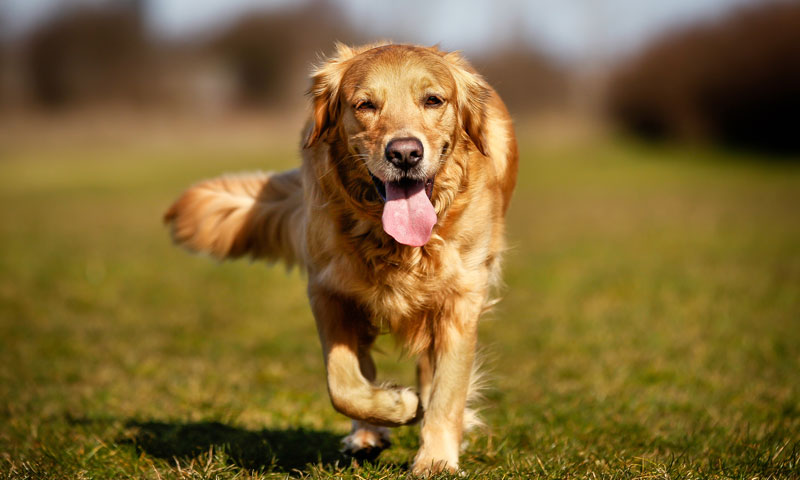
\includegraphics[height=0.2\paperheight]{perro.jpg}
                    \caption{Perro corriendo}
                    \label{fig:perro}
                \end{figure}
            \end{column}
            \begin{column}{0.5\textwidth}
                Sin embargo, es necesario añadir al \emph{preámbulo} el comando
                {\scriptsize \mint{latex}|\setbeamertemplate{caption}[numbered]|}
                para que las figuras queden numeradas.
            \end{column}
        \end{columns}

    \end{frame}

    %%%%%%%%%%%%%%%%%%%%%%%%%%%%%%%%%%%%%%%%%%%%%%%%%%%%%%%%%%%%%%%%%%%
    \begin{frame}[fragile]{Subfiguras}
        \framesubtitle{Paquete \emph{subcaption}}
        Insertar varias figuras, también funciona igual que siempre.
        \begin{figure}
            \centering
            \begin{subfigure}[b]{0.4\textwidth}
                \centering
                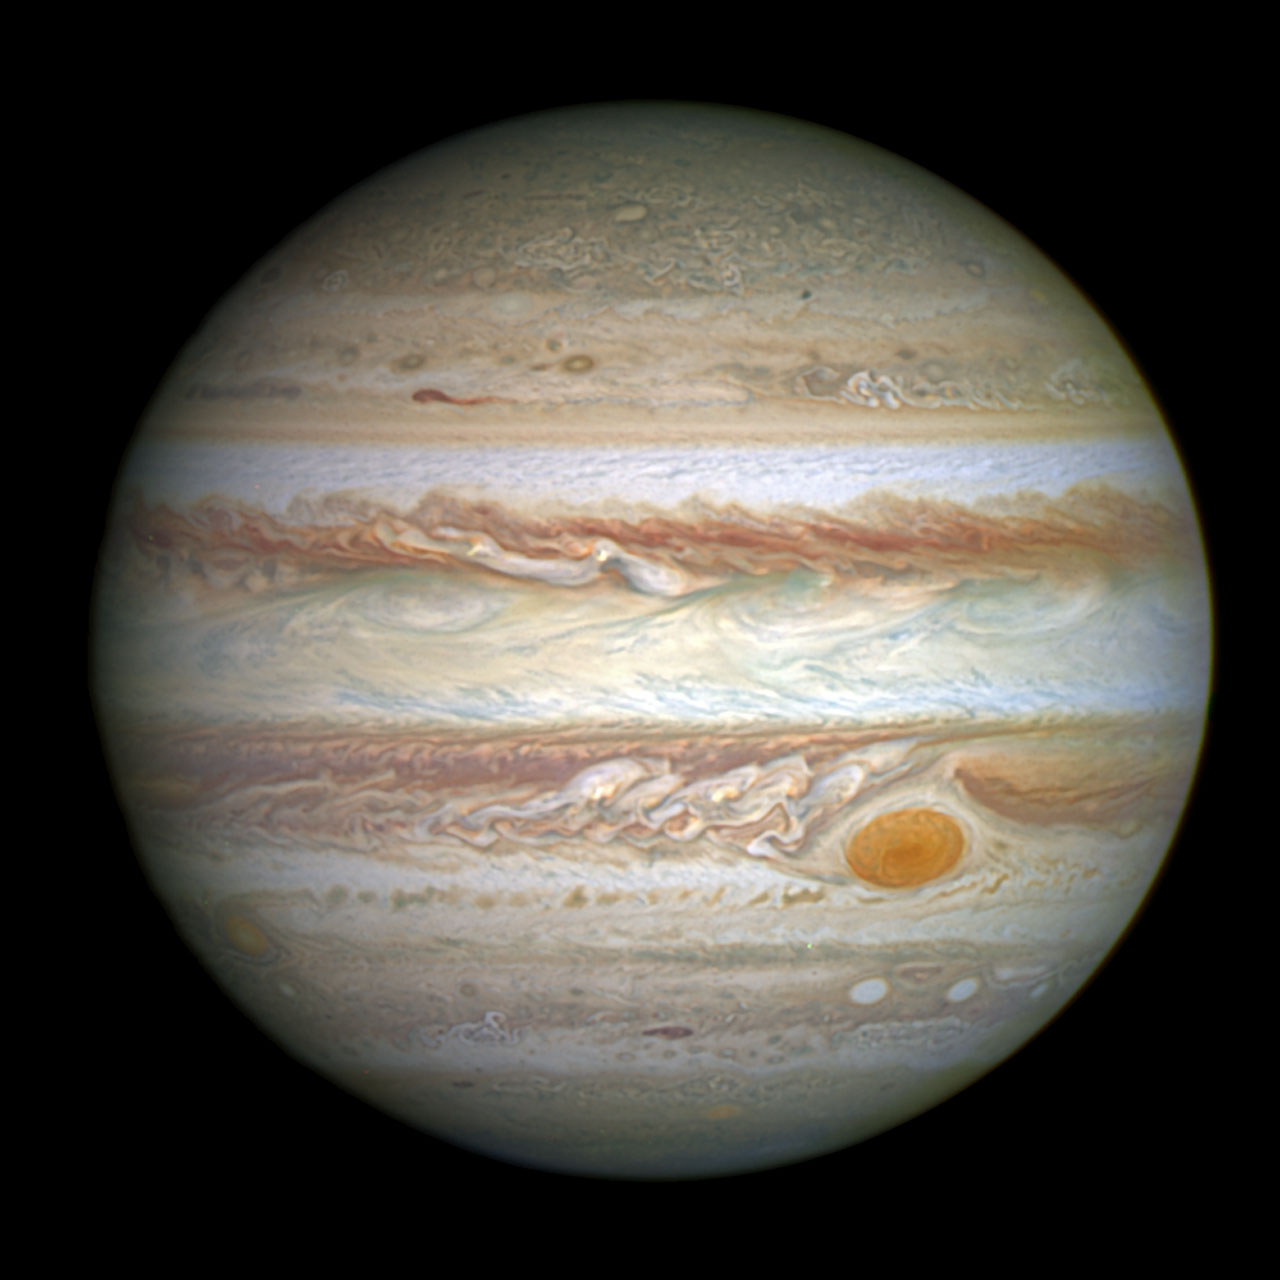
\includegraphics[width=2cm, height=2cm]{jupiter.jpg}
                \caption{Júpiter}
                \label{fig:jupiter}
            \end{subfigure}
            \hspace{1cm}
            \begin{subfigure}[b]{0.4\textwidth}
                \centering
                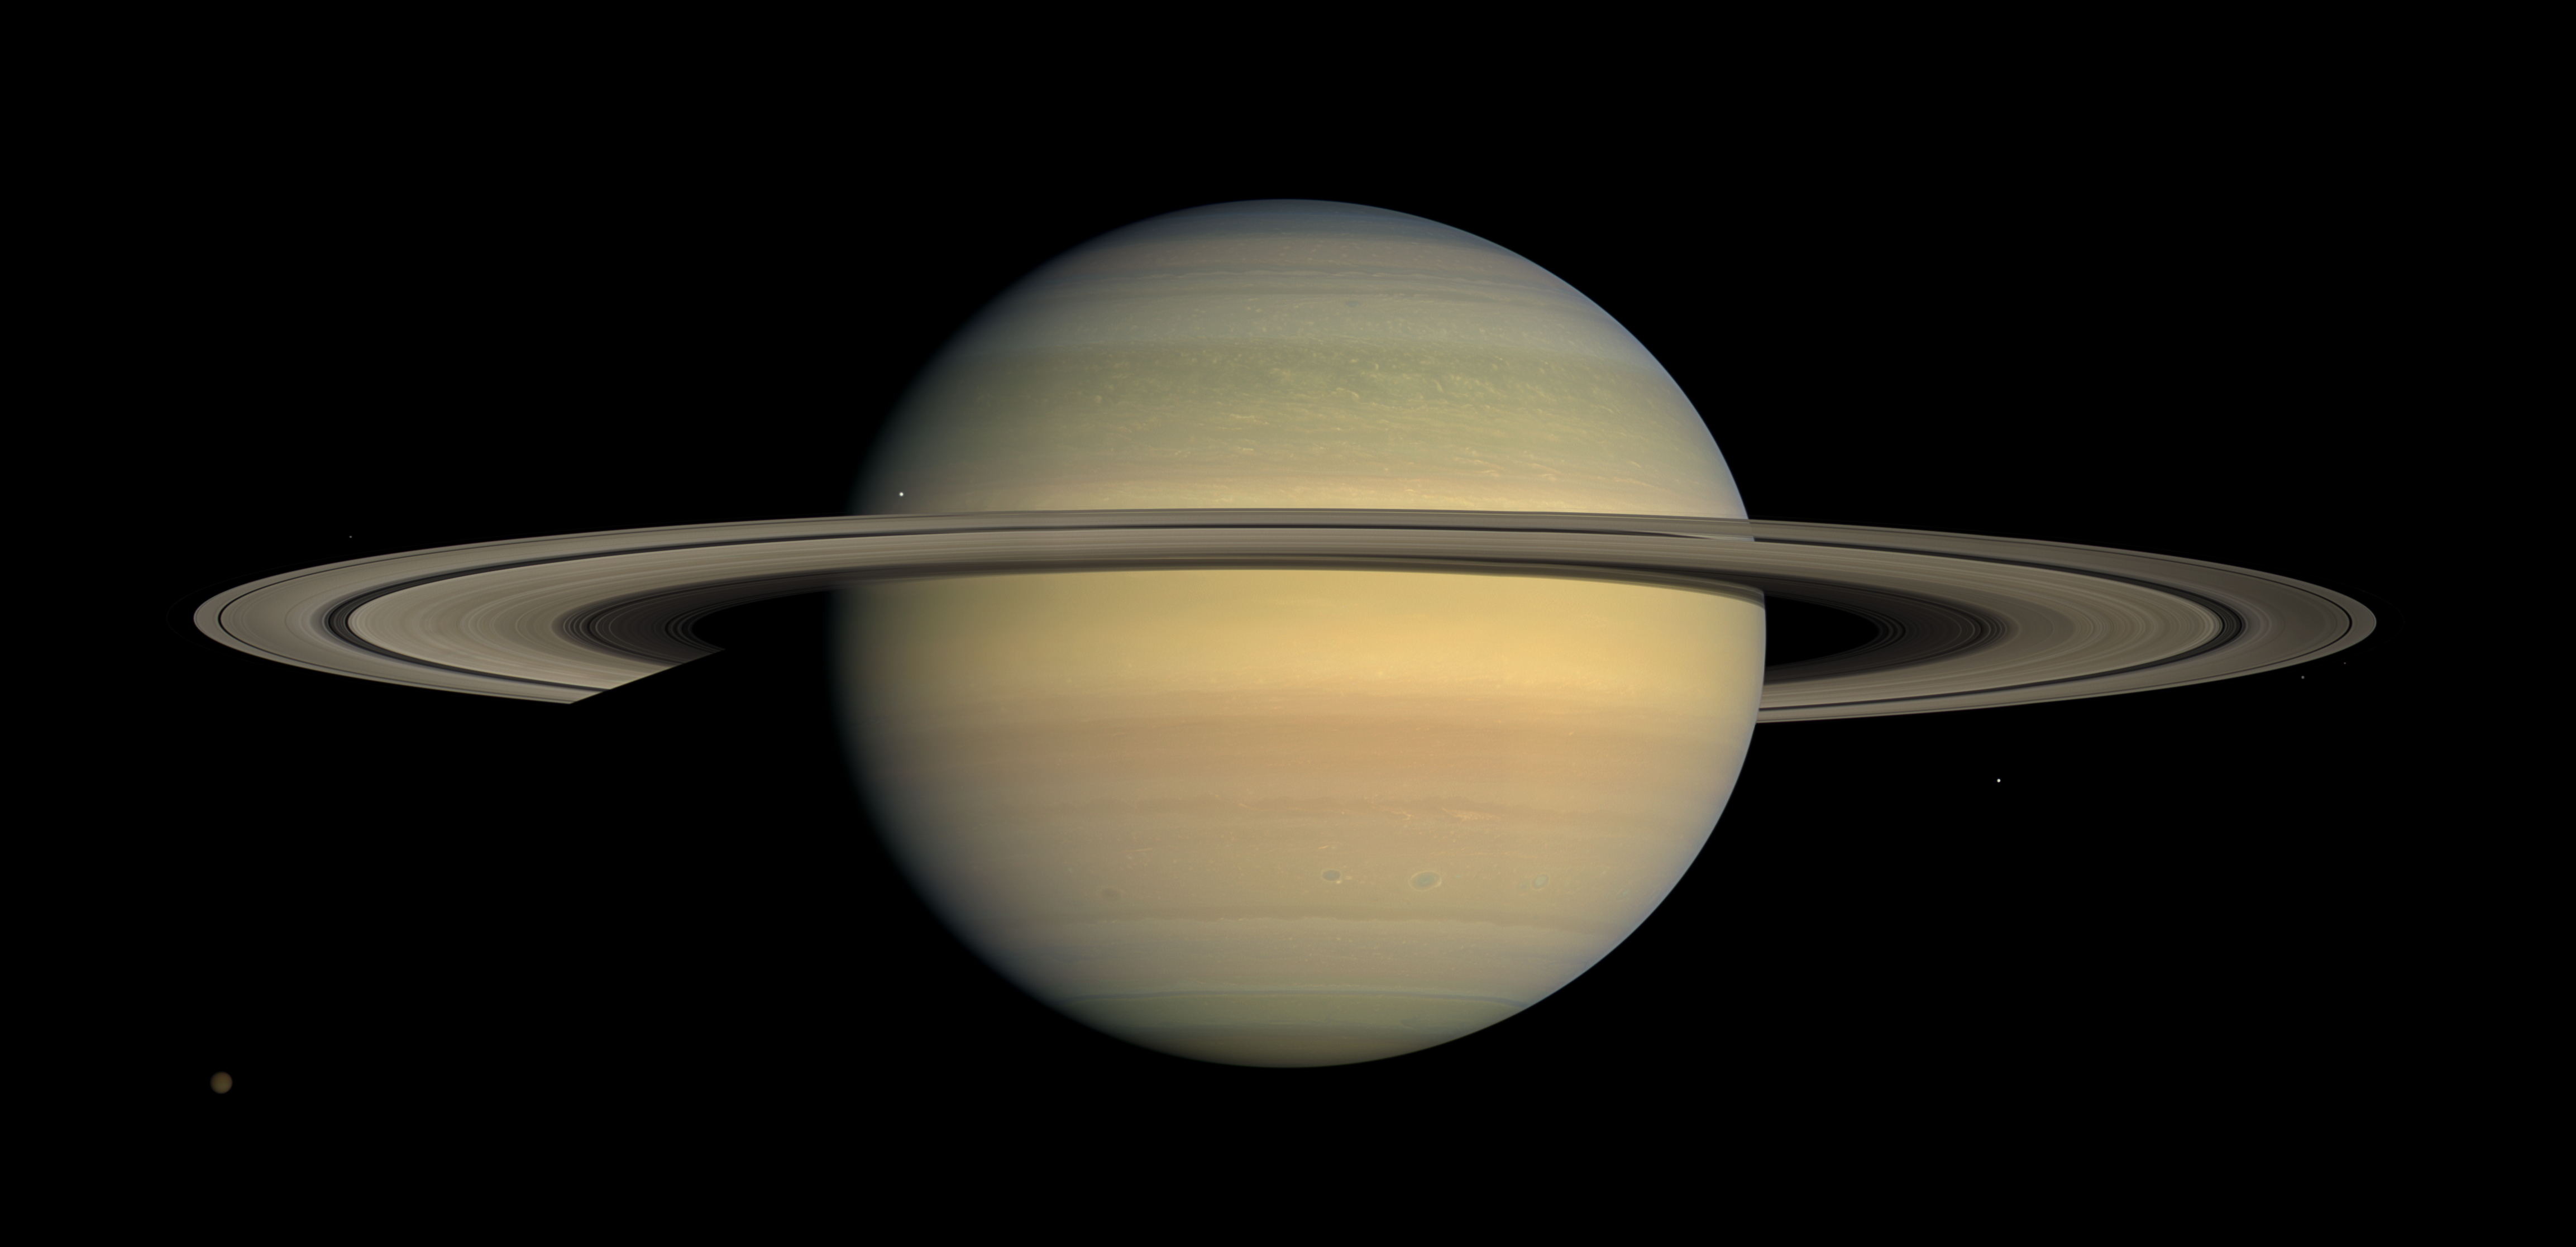
\includegraphics[width=3.5cm, height=2cm]{saturno.jpg}
                \caption{Saturno}
                \label{fig:saturno}
            \end{subfigure}\\
            \begin{subfigure}[b]{0.4\textwidth}
                \centering
                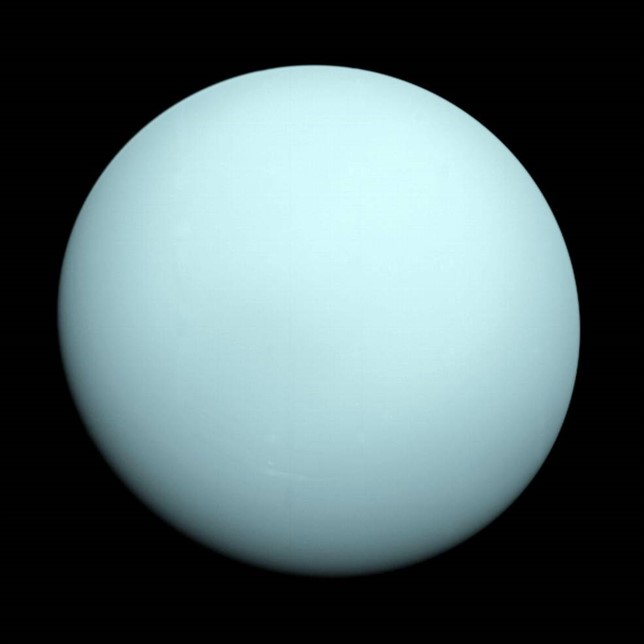
\includegraphics[width=2cm, height=2cm]{urano.jpg}
                \caption{Urano}
                \label{fig:urano}
            \end{subfigure}
            \hspace{1cm}
            \begin{subfigure}[b]{0.4\textwidth}
                \centering
                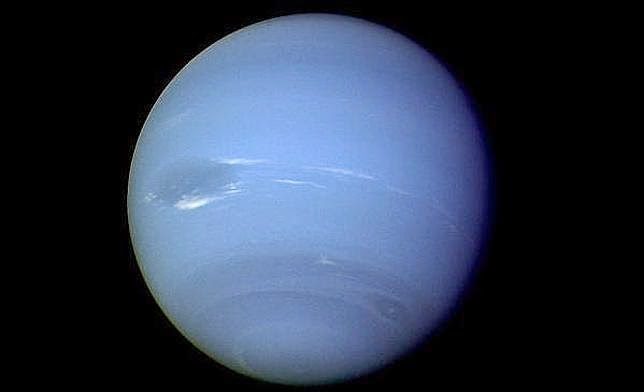
\includegraphics[width=3.5cm, height=2cm]{neptuno.jpg}
                \caption{Neptuno}
                \label{fig:neptuno}
            \end{subfigure}
            \caption{Planetas gaseosos}
            \label{fig:planetas}
        \end{figure}
    \end{frame}

    %%%%%%%%%%%%%%%%%%%%%%%%%%%%%%%%%%%%%%%%%%%%%%%%%%%%%%%%%%%%%
    \begin{frame}[fragile]{Resaltando cosas importantes}
        \justifying
        En una presentación es \alert{buena práctica} remarcar puntos importantes para llamar
        la \alert{atención} de la audiencia.
        \begin{itemize}
            \justifying
            \item Para resaltar una palabra o una frase, el comando {\color{mygreen}\verb|\alert{}|} cambia
            el estilo del texto entre llaves. Cómo luzca ese texto depende del tema usado.
            \item Para resaltar un párrafo con conceptos, definiciones, teoremas o ejemplos, la mejor opción
            es utilizar una caja. Existen tres tipos de cajas, y es decisión del autor cuál usar:
            \begin{itemize}
                \item \verb|block|
                \item \verb|alertblock|
                \item \verb|examples|
            \end{itemize}
        \end{itemize}
    \end{frame}

    %%%%%%%%%%%%%%%%%%%%%%%%%%%%%%%%%%%%%%%%%%
    \begin{frame}[fragile]{Resaltando cosas importantes}
        \begin{minipage}{0.5\textwidth}
            \begin{block}{Primer tipo de caja: block}
                Contenido relevante para resaltar.
            \end{block}
        \end{minipage}
        \begin{alertblock}{Segundo tipo de caja: alertblock}
            Contenido relevante para resaltar.
        \end{alertblock}
        \begin{examples}
            Tercer tipo de caja: examples. \\ 
            Contenido relevante para resaltar. El título ``Examples''
            es fijo, para modificar el idioma hay que modificar los archivos
            fuente de \texttt{beamer}, lo cual hice para esta presentación.
        \end{examples}
    \end{frame}
    %%%%%%%%%%%%%%%%%%%%%%%%%%%%%%%%%%%%%%%%%%
    \begin{frame}[fragile]{Temas}
        \begin{itemize}
            \justifying
            \item Es muy fácil usar un \href{https://hartwork.org/beamer-theme-matrix/}{\textcolor{blue}{\underline{tema}}} diferente en la presentación. Simplemente hay que usar el comando
            {\color{mygreen}\verb|\usetheme{|}\verb|nombre del tema|{\color{mygreen}\verb|}|} en el
            \textsl{preámbulo}.
            \item Los temas pueden combinarse con un \textbf{color de tema}, con el comando {\color{mygreen}\verb|\usecolortheme{|}\verb|nombre del color|{\color{mygreen}\verb|}|}.
            Esto cambia el color usado para distintos elementos de la presentación. {\color{mygreen}\verb|\usecolortheme|} debe ir
            siempre después que  {\color{mygreen}\verb|\usetheme|}
        \end{itemize}
    \end{frame}    

    %%%%%%%%%%%%%%%%%%%%%%%%%%%%%%%%%%%%%%%%%%%%%
    \begin{frame}[fragile]{Tipo y tamaño de fuente}
        \begin{minipage}{0.93\paperwidth}
        \begin{itemize}
            \justifying
            \item El \textbf{tamaño de fuente} puede pasarse como parámetro a la clase \texttt{beamer} al inicio del documento.
            Los tamaños de fuente disponibles son 8pt, 9pt, 10pt, 11pt (por defecto), 12pt, 14pt, 17pt y 20pt.
            \item Para cambiar los tipos de fuente se utiliza un comando que ya vimos antes:  {\color{mygreen} \verb|\usefonttheme{}|}.
            Los tipos de fuente disponibles son: \texttt{default}, \texttt{professionalfonts}, \texttt{serif}, \texttt{structurebold},
            \texttt{structureitalicserif} y \texttt{structuresmallcapsserif}.
        \end{itemize}
        \end{minipage}
    \end{frame}
    
    %%%%%%%%%%%%%%%%%%%%%%%%%%%%%%%%%%%%%%%%%%%%%
    \begin{frame}[fragile]{Columnas}
        En ocasiones, la información en una presentación luce mejor en un formato de dos columnas. Para eso existe el ambiente
        \textsl{columns}.
        \vspace{5mm}
        \begin{center}
            \begin{minipage}{0.89\textwidth}
                \inputminted[fontsize=\tiny, frame=single]{latex}{two_columns.tex}
            \end{minipage}
        \end{center}
    \end{frame}

    %%%%%%%%%%%%%%%%%%%%%%%%%%%%%%%%%%%%%%%%%%%%%
    \begin{frame}{Diapositiva con dos columnas}
        Texto \cite{einstein}.
        \begin{columns}[totalwidth=\textwidth]
            \begin{column}[t]{0.5\textwidth}
            \centering
            \textsc{Ecuación de Schrödinger en una columna}.
            \vspace{0.5cm}
            \begin{equation*}
                -\frac{\hbar^2}{2m}\nabla^2\psi + V\psi =  i\hbar\frac{\partial \psi}{\partial t}
            \end{equation*}
            \end{column}
            \vrule{}
            \begin{column}[t]{0.5\textwidth}
                \centering
                \emph{\textrm{Imagen de un gato en la otra}}\\ [2ex]
                \centering
                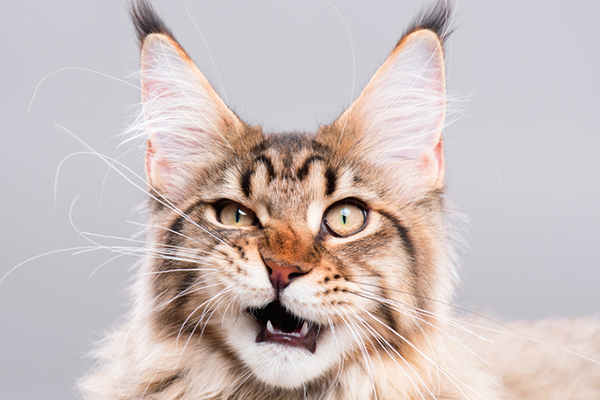
\includegraphics[width=0.8\linewidth]{gato.jpeg}
            \end{column}
        \end{columns}        
    \end{frame}

    %%%%%%%%%%%%%%%%%%%%%%%%%%%%%%%%
    \begin{frame}[fragile]{Minipáginas}
        Existe el ambiente \cmdbs{minipage}, para manipular
        elementos en un espacio reducido. \\ [3ex]
        \begin{center}
            \begin{minipage}{0.45\textwidth}        
                \begin{minted}[frame=single]{latex}
\begin{minipage}{width}
    % Contenido
\end{minipage}
                \end{minted}
            \end{minipage}
        \end{center}
    \end{frame}

    \begin{frame}{Referencias}
        \printbibliography
    \end{frame}
\end{document}